\documentclass[a4paper]{IEEEtran}
%\usepackage{a4wide}
\usepackage{graphicx}
\usepackage{caption}
\usepackage{subcaption}
\usepackage{eurosym}
%%\setlength{\parindent}{0in}

\title{IN4150 Distributed Algorithms\\Randomized Byzantine Agreement}

\author{\IEEEauthorblockN{Peter van Buul}
1359347\\
\and
\IEEEauthorblockN{Rogier Slag}
1507761\\
}
\begin{document}
\maketitle
\begin{center}
\today
\end{center}

\section{Test setup}

Due to the work of the authors, we had access to quite powerful blade servers we were able to use to run a large set of tests fairly quickly.
The blade servers were equipped with 24 processor cores and used 512 GB of memory.
Local SSD storage was available. 
Every test scenario was run at least 20 times to average the randomness in the algorithm.

\section{Algorithm setup}

The algorithm was implemented in the usual fashion.
Failing nodes were also implemented.
A node could fail in several aspects:
during the algorithm startup, a node which should fail would perform a coin flip.
In one case the node would never send a message, whereas in the other case it would send random messages.
In case the node would send a random message,
it would perform a coin flip to determine whether to send a 0 or a 1.
\\
\\
Although during the initialization of the run the information of the failing nodes was present,
the separate nodes did not possess any of this information.
This ensured the algorithm would perform as intended (random failures and not knowing who to trust).
\\
\\
A number of assumptions was made in the program:
first of all a message is never lost in transit (it is either sent or not sent).
Secondly the links do not have any data corruption risk and do not tamper with the messages.
Finally the nodes do not have any other knowledge than they have sent to each other and the total number of processes.

\section{Test runs}

During the test runs we observed the algorithm to converge quite quickly when the number of traitors is much less then $\frac{1}{5}n$.
Whenever the relation $f < \frac{n}{10}$ the algorithm never used more than 10 rounds to decide,
which would happen in a matter of seconds (actually faster, but the verbose logging significantly slowed down execution, but this logging was needed to check the process of the algorithm).
\\
\\
When the number of failing processes became in the range of $\frac{n}{10} < f < \frac{n}{5}$ the required number of rounds would grow very fast.
Since this difference is interesting, we decided to plot the data we obtained (using the averages) and determine whether a relation could exist.
The following figure was obtained (after leaving out some scatter points to improve readability).

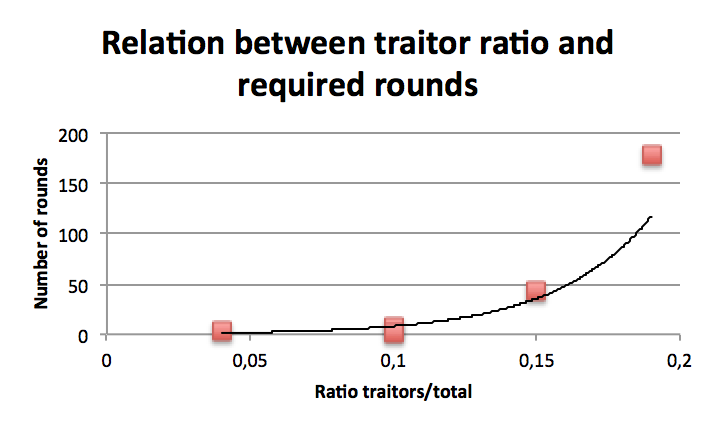
\includegraphics[scale=0.7]{relationship.png}

Analysis determined the relationship between $\frac{f}{n}$ and the number of rounds required was exponential.
A trend line for exponential growth was added to the graph to show this.
\\
\\
Once a ratio of $\geq \frac{f}{n}$ was obtained, this image would shift.
Although some situations would remain solvable, this would be non-deterministic.
This was opposed to the previous situations, which in our tests always terminated with some decision.
\\
\\
We decided to stop a test if it had reached 1500 rounds without reaching consensus.
As would be expected, this cut-off point was sometimes reached for a test case,
but was not reached when the same test was rerun. 
\\
\\
To summarize, the tests we ran supported the theory the algorithm worked well in the first range, encountered performance slowdown in the second range and would sometimes terminate in the final range (and sometimes not).
All of this in in accordance with the respective theory on the algorithm.

\section{Results}

From a number of tests we have saved the actual results such that someone could verify how the processes decided on the end value.
A number of five representative tests was chosen.
\\
\\
The first test used 100 processes, of which 10 were faulty.
The second test used 100 processes, of which 15 were faulty.
In the third test, the maximum number of 19 processes (of the hundred) behaved incorrectly.
Next a larger set was used; 250 processed of which 10 were erroneous.
In the final test a total of 250 processes was used with 25 exhibiting failures.
\\
\\
An attempt was made to use several parallel servers since the JVM encountered issues with the thread count.
However this hardware was not available for testing, therefore this attempt was abandoned.
\\
\\
These test results can be obtained from https://gist.github.com/rogierslag/07b67196e8343035907a

\end{document}
